\chapter{Tutorial}

\section{Starting Kobold}

Start the Kobold server by entering the following into the console:\par
java -Djavax.net.debug=all -Dkobold.server.messageStore=bla.xml \\
-Djava.protocol.handler.pkgs=com.sun.net.ssl.internal.www.protocol \\
-Djavax.net.ssl.keyStore=/home/eclipse/kobold.common/scripts/keystore \\
-Djavax.net.ssl.keyStorePassword=kobold1 \\
-Djavax.net.ssl.trustStore=/home/eclipse/kobold.common/scripts/truststore\\
 -Djavax.net.ssl.trustStorePassword=kobold1 SecureKoboldWebServer 23232\par
Note: You will have to change the paths in the command above to make 
them fit your structure.\par

Start Eclipse and select 'Run...' in the 'Run' menu. In the opening dialog 
double-click 'Run-time Workbench'. A new configuration is created which you 
can name as you wish (see \ref{run}). 

\begin{figure}[h!]
\begin{center}
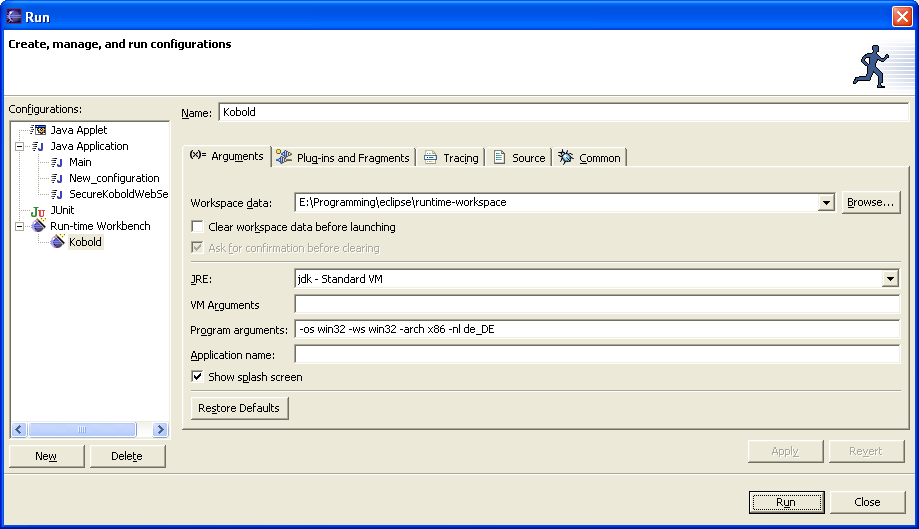
\includegraphics[width=15cm]{run.png}
   \caption{This is how your buildpath should look like}
\label{run}
\end{center}
\end{figure}\par

Enter the following VM Arguments: \par

-Djavax.net.debug=all\\
-Djava.protocol.handler.pkgs=com.sun.net.ssl.internal.www.protocol\\
-Djavax.net.ssl.keyStore=/home/eclipse/kobold.common/scripts/keystore\\
-Djavax.net.ssl.keyStorePassword=kobold1\\
-Djavax.net.ssl.trustStore=/home/eclipse/kobold.common/scripts/truststore\\
-Djavax.net.ssl.trustStorePassword=kobold1 \par

Confirm with 'Run'.\par

A new Eclipse instance will open called Kobold Productline.

\section{Checking out a product(line)}

In the File menu select 'New' and then 'Kobold PLAM Project'. The Kobold wizard opens.
Enter the name of the project you want to create (see \ref{wizard1}).

\begin{figure}[h!]
\begin{center}
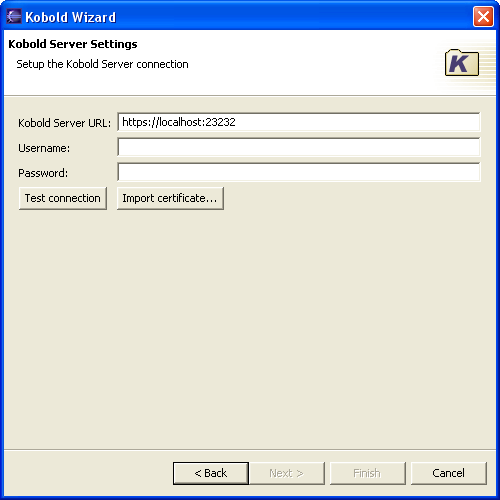
\includegraphics[width=10cm]{wizard1.png}
   \caption{Kobold wizard}
\label{wizard1}
\end{center}
\end{figure}\par

After that enter the url of your Kobold server, your username and password (see \ref{wizard2}).

\begin{figure}[h!]
\begin{center}

\includegraphics[width=10cm]{wizard2.png}
   \caption{Kobold wizard}
\label{wizard2}
\end{center}
\end{figure}\par

In the last step you have to choose the productline (see \ref{wizard3}).

\begin{figure}[h!]
\begin{center}
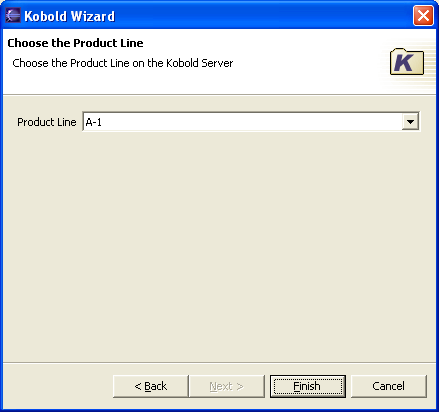
\includegraphics[width=10cm]{wizard3.png}
   \caption{Kobold wizard}
\label{wizard3}
\end{center}
\end{figure}\par

A new project has been created. You can open the different views through the Window menu
and 'show view'. 